% !TEX root = diplomarbeit.tex
\chapter{Marketing}
\renewcommand{\kapitelautor}{Autor: Markus Kaiser}

%%%%%%%%%%%%%%%%%%%%%%%%%%%%%%%%%%%%%%%%%%%%%%%%%%%%%%%%%%%%%%%%%%%%%%%%%%%%%%%
\section{Allgemein}
Im folgenden Kapitel wird beschrieben, mit welchen Mitteln und mit welcher Effektivität
das Projekt Hovering Steward vermarktet wurde. Unter anderem werden diverse Marktanalysen
aber auch Marketing-Strategien und deren Anwendung erläutert.

  \subsection{Marktanalysen}
    \subsection*{SWOT-Analyse}
    Mithilfe der SWOT-Analyse wird der aktuelle Zustand eines Unternehmens, oder in unserem Fall Projektes, analysiert um anschließend eine von vier möglichen Strategien
    für den weiteren Verlauf des Unternehmens zu erarbeiten. Es werden Stärken, Schwächen, Möglichkeiten und Risiken evaluiert, wobei sich jeweils Stärken und Schwächen, und
    Möglichkeiten und Risiken gegenüberstehen. Die vier Begriffe auf englisch übersetzt \textbf{S}trengths, \textbf{W}eaknesses, \textbf{O}pportunities und \textbf{R}isks
    ergeben dadurch das Akronym SWOT.

    \begin{figure}[H]
      \begin{centering}
      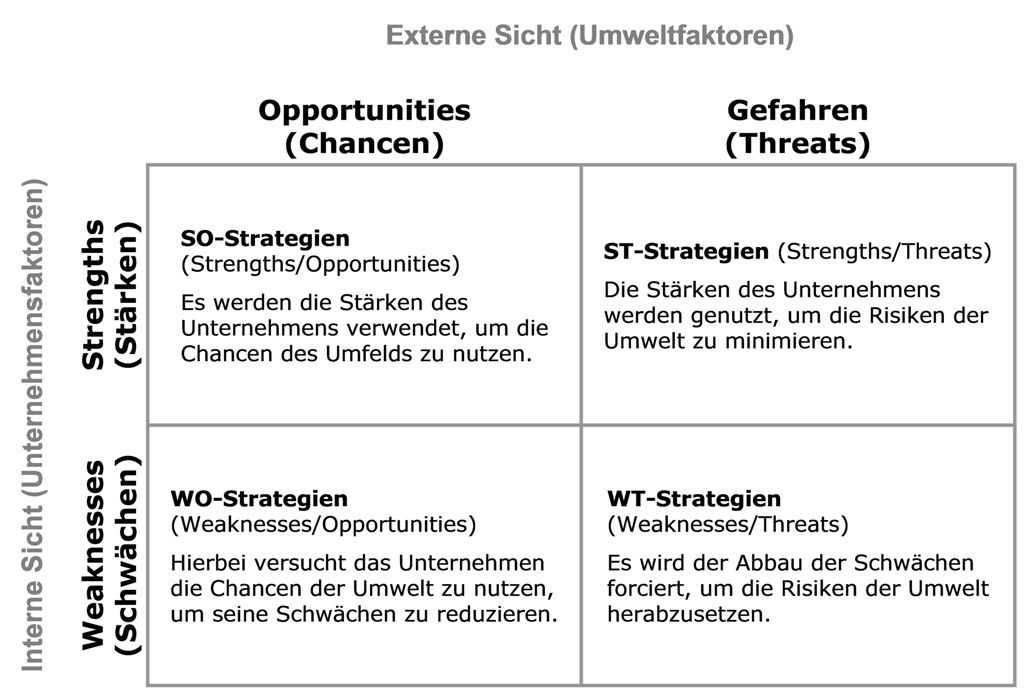
\includegraphics[width = 1\textwidth]{Bilder/swot.jpg}
      \par\end{centering}
      \caption[SWOT-Analyse Grafik]{SWOT-Analyse Grafik\cite{pic_swot}}
      \label{swot}
    \end{figure}

    \subsection*{Die vier Strategien:}
    \begin{itemize}
      \item \textbf{SO-Strategie}
      Die Stärken des Unternehmens werden hervorgehoben und mit den Möglichkeiten verknüpft. Macht ein Unternehmen beispielsweise hohe Umsätze in Industrieländern und hat
      genügend finanzielle Mittel, wird expandiert und ein neuer Standort in einem weiteren Industrieland aufgebaut.

      \item \textbf{ST-Strategie}
      Auch hier werden die Stärken des Unternehmens genutzt, allerdings um bestehende Risiken einzuschränken oder zu entfernen. Besteht die Gefahr, dass die Konkurrenz
      einen höheren Marktanteil erlangt, kann das Unternehmen beispielsweise durch eine sehr gute Marketingabteilung neue Produkte herstellen, die dies verhindern.

      \item \textbf{WO-Strategie}
      Hierbei wird versucht, die Schwächen eines Unternehmens als Chance zu sehen sich weiterzuentwickeln. Erzielt ein gewisses Produkt nicht die erwarteten Gewinne,
      können durch neue Lösungsansätze neue Erfahrungen gewonnen werden, die nach Erfolg auch auf andere Produkte angewendet werden können.

      \item \textbf{WT-Strategie}
      Die Schwächen des Unternehmens werden näher betrachtet, um beim Versuch diese zu dezimieren, gleichzeitig Risiken einzugrenzen. Diese Strategie kann sehr hilfreich
      sein, wenn das Unternehmen sich auf dem Markt schwer über Wasser halten kann.
    \end{itemize}

    \subsection*{Portfolioanalyse nach Boston Consulting Group}
    Die Definition laut {"Boston Consulting Group"\cite{portfolioanalyse}} beschreibt die Portfolioanalyse wie folgt:
    "Das BCG-Portfolio erlaubt eine Bewertung strategisch relevanter Geschäftseinheiten auf Basis zukünftiger Gewinnchancen (Marktwachstum) und der
    gegenwärtigen Wettbewerbsposition (relativer Marktanteil)."
    Anders gesagt: Diese Analyse hilft dabei Teile eines Unternehmens wie Produkte oder Dienstleistungen
    nach Kosten und Ertrag einzuschätzen und in vier Kategorien zu unterteilen.

    \begin{figure}[H]
      \begin{centering}
      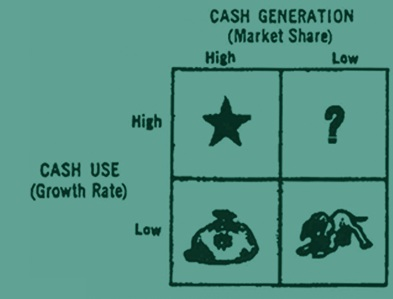
\includegraphics[width = 1\textwidth]{Bilder/portfoliomatrix.jpg}
      \par\end{centering}
      \caption[Portfoliomatrix]{Portfoliomatrix\cite{pic_matrix}}
      \label{matrix}
    \end{figure}

    \begin{itemize}
      \item Die \textbf{Cashcow} ist ein Produkt des Unternehmens, welches sich bereits lange Zeit auf dem Markt hält und dadurch hohe Gewinne erziehlt. Durch die
      erarbeitete hohe Position auf dem Markt decken sich ihre Kosten durch den Gewinn selbst. Die Cashcow stellt zudem die Basis für die Weiterentwicklung anderer
      Produkte dar.

      \item Der \textbf{Superstar} ist ein Produkt mit den besten Aussichten. Es erzielt bereits nach kurzer Zeit auf dem Markt hohe Gewinne. Um den Marktanteil
      zu halten, muss jedoch viel in dieses Produkt investiert werden. In der Regel geschieht dies durch die Überschüsse, die die Cashcow abwirft.

      \item Ein \textbf{Poor Dog} ist ein weniger erfolgreiches Produkt. Da es nach hohen Investitionen und langer Zeit auf dem Markt keine nennenswerte
      Gewinne erbracht hat, ist es ratsam zu überlegen, ob weiter investiert, oder die Produktion gestoppt wird.

      \item Als \textbf{Questionmarks} werden die Produkte bezeichnet, bei denen sich noch nicht eindeutig gezeigt hat, in welche Richtung sie sich entwickeln werden.
      Es steht offen ob sie zu einem Superstar, oder einem Poor Dog werden. Diese Tatsache macht es schwer zu entscheiden, ob weiter in sie investiert, oder das Produkt
      verkauft wird.
    \end{itemize}

    \subsection*{SWOT-Analyse von Hovering Steward}
    Da sich die Portfolioanalyse nach der Boston Consulting Group eher für Unternehmen eignet, die mehrere Produkte oder Dienstleistungen anbieten war sie für das Projekt
    Hovering Steward weniger relevant. Aus diesem Grund wurde eine SWOT-Analyse durchgeführt.

    \begin{figure}[H]
      \begin{centering}
      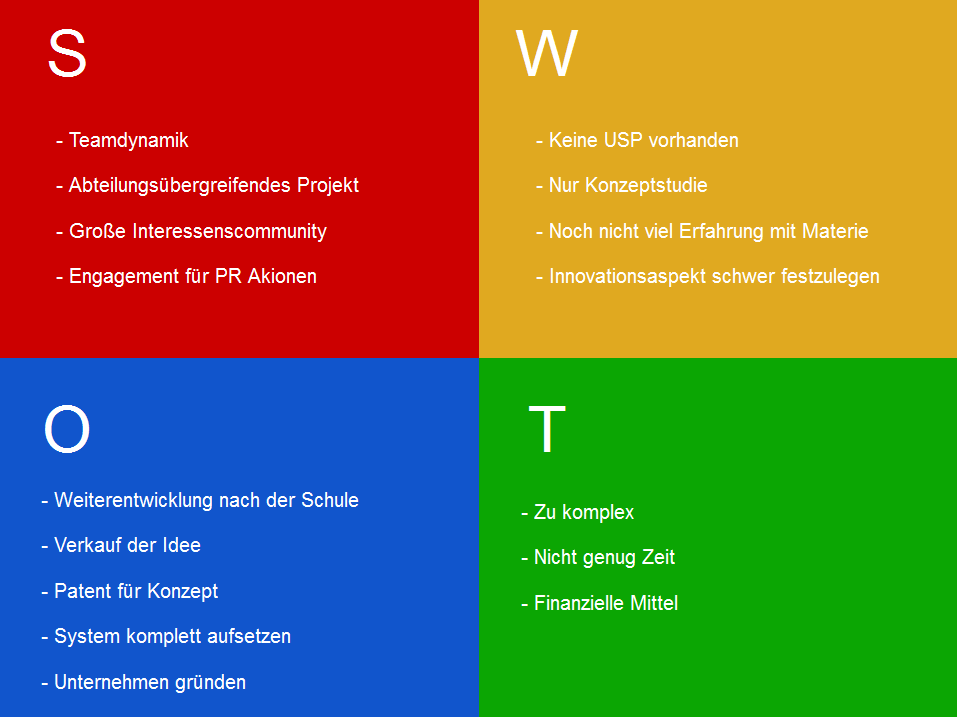
\includegraphics[width = 1\textwidth]{Bilder/hovi_SWOT.png}
      \par\end{centering}
      \caption{SWOT-Analyse von Hovering Steward}
      \label{hoviswot}
    \end{figure}

  \subsection{Marketing-Strategie}
  Aus der SWOT-Analyse ging hervor, dass unsere Schwächen großteils darin lagen, unser Projekt nur schwer präsentieren zu können, da das Hauptziel das Entwickeln
  einer Konzeptstudie, keines fertigen Produktes ist. Außerdem ergaben Kostenabschätzungen, dass das Testen der Konzepte einen hohen finanziellen Aufwand mit sich bringen
  würde. Aus diesen beiden Erkenntnissen entstand das Vorhaben, das Projekt sehr aktiv an die Öffentlichkeit zu bringen, um zum einen zu intensiv Fortschritte im Projekt
  für Außenstehende als ersichtlich zu gestalten und zum anderen dadurch in Kontakt mit potentiellen Sponsoren und Partner zu geraten, und folglich das Budget des Projekts
  decken zu können. Diese Vorgehensweise fällt unter die Kategorie der WT-Strategie, auf Basis der SWOT-Analyse.

    \subsection*{Corporate Design}
    Um einen professionellen Eindruck bei Internetauftritten und Events zu vermitteln, wurde ein Corporate Design entwickelt.
    Das Corporate Design diente als Guideline für das gestalten jeglicher visueller Verweise auf die Diplomarbeit Hovering Steward.
    Es wurden Eigenschaften für das Logo, bestimmte Farben und zu verwendende Fonts festgelegt.
    Somit war es möglich dem Projekt ein einheitliches Auftreten in der Öffentlichkeit, und damit einen Wiedererkennungswert zu verleihen.

    \subsection*{Visitenkarten}
    Um die Außenwelt auf unser Projekt aufmerksam zu machen, wurden Visitenkarten entworfen, die sich von anderen Projekten abheben.
    Sie sollten sowohl die notwendige Information auf den ersten Blick vermitteln, als auch ein anspruchsvolles Design repräsentieren. Aus dem Vorhaben,
    mit Marketing Transparenz in unserem Projekt zu schaffen entstand die Idee, die Karten zum Teil transparent zu gestalten.
    Das Ergebnis war folgendes:

    \begin{figure}[H]
      \begin{centering}
      
\includegraphics[width = 1\textwidth]{Bilder/visitenkarte.jpg}
      \par\end{centering}
      \caption{Visitenkarte von Hovering Steward}
      \label{visitenkarte}
    \end{figure}

    \subsection*{Blog}
    Der Blog war die wichtigste Komponente für das Veröffentlichen von akuellen Informationen. Es wurde Wert darauf gelegt,
    in regelmäßgen Abständen, aktuelle Inhalte über den Projektverlauf zu veröffentlichen. Die Zielgruppe waren primär junge TechnikerInnen,
    die sich für Drohnen, oder allgemein für Robotik interessierten. Alles zur Entwicklung des Blogs ist in Kapitel 1.3 angeführt.

    \subsection*{Wettbewerbe}
    Hovering Steward hat an einer Vielzahl an Wettbewerben teilgenommen, auf welche im Kapitel Public Relations näher eingegangen wird.
    Folgende Vorteile waren eine Motivation, eine Bewerbung für diese einzuschicken:

    \begin{itemize}
      \item \textbf{Teamdynamik}

      Bei einer Präsentation vor fremdem Publikum war ein professionelles Auftreten, gute Planung und vorallem Koordination gefragt.
      Diese Auftritte wurden als Chancen genutzt, die Dynamik im Team weiterzuentwickeln, als auch Präsentationstechniken für
      die Endpräsentation zu trainieren.

      \item \textbf{Unterstützung}

      Ein weiterer Vorteil war, dass durch die Teilnahme an Wettbewerben von den veranstaltenden Unternehmen, Unterstützung geboten wurde. Nicht nur im finanziellen
      Bereich, sondern auch durch Workshops oder ähnliche hilfreiche Events.

      \item \textbf{Marketing}

      Nicht zuletzt waren Wettbewerbe ein wichtiger Teil des Marketings, da sich unsere Idee nicht nur durch Präsentationen verbreiten ließ,
      sondern auch in den Sozialen Medien und auf den Webseiten der Veranstalter erwähnt wurde.

    \end{itemize}


%%%%%%%%%%%%%%%%%%%%%%%%%%%%%%%%%%%%%%%%%%%%%%%%%%%%%%%%%%%%%%%%%%%%%%%%%%%%%%%
\section{Public Relations}

  \subsection{Wettbewerbe, Events, Präsentationen}

    \subsection*{Jugend Innovativ}
    {JugendInnovativ\cite{jugendinnovativ}} ist einer der bekanntesten Bewerbe, die Schul- und Diplomarbeitsprojekte
    unterstützten. Wie der Name schon sagt, legt die Jury hierbei sehr großen Wert auf den innovativen
    Aspekt der Projektidee. Zu diesem Zweck haben wir eine eigene Executive Summary verfasst, die nicht
    nur auf den technischen Hintergründen basiert, sondern hervorhebt, was unser Projekt einzigartig
    macht. Unser Team hat das Halbfinale von JugendInnovativ erreicht, und somit eine finanzielle Unterstützung
    zugesagt bekommen.

    \subsection*{Bosch - Technik fürs Leben Preis}
    Die Bosch-Gruppe Österreich ist Initiator des jährlichen Wettbewerbs {"Technik fürs Leben"\cite{bosch}}. Es werden Österreichs
    größte Talente des technisch orientierten Nachwuchses gesucht. Projekte werden von einer Experten-Jury bewertet,
    der Hauptpreis is das Angebot für ein Praktikum bei der Bosch Gruppe Österreich.

    \subsection*{Accenture HTL Challenge}
    Der Managementberatungs-, Technologie- und Outsourcing Dienstleister {Accenture\cite{accenture}} veranstalten jedes Jahr die Accenture HTL Challenge,
    bei der Projekte und Diplomarbeiten von technischen Schulen, rund um das Thema Informationstechnologie gesucht werden.
    Die Teams treten durch Präsentationen vor einer Jury gegeneinander an. Neben dem Wettbewerb werden den Teilnehmern außerdem
    Unterstützungen wie Coachings und Beratungen von Experten angeboten. Aufgrund des Umfangs dieses Wettbewerbs haben wir uns entschieden an diesem teilzunehmen,
    um das Projekt auch hier an die Öffentlichkeit zu bringen und bei Gelegenheit Kontakte zu knüpfen. Hovering Steward schaffte es ins Finale der
    Accenture HTL Challenge.

    \subsection*{ITs Project Award}
    Der {ITs Project Award\cite{its}} ist ein Event der FH Salzburg. Projekte und Diplomarbeiten aus den Bereichen Informations- und Kommunikationstechnologie
    können eingereicht werden, aufsteigende Teams treten in einem Finale gegeneinander an und müssen ihr Projekt präsentieren. Bewertet werden die
    Teams von einer Expertenjury nach Kriterien wie Kreativität, Innovationsaspekt oder wirtschaftlicher Relevanz.
    Auch in diesem Bewerb erreichte Hovering Steward das Finale.

    \subsection*{Invasion der Drohnen}
    Zu Begin der Diplomarbeit haben wir versucht möglichst viel über die Entwicklung und den Einsatz von Drohnen zu erfahren.
    Der Vortrag {Invasion der Drohnen\cite{invasionderdrohnen}}, mit anschließender Diskussion zum Thema "Entwicklung von Drohnen, Einsatzgebiete und rechtliche Einschränkungen" brachte
    uns viele neue Informationen, wie der Umgang mit unbemannten Flugobjekten, speziell in Österreich gehandhabt werden.

    \subsection*{European Conference on Educational Robotics}
    Über den Wettbewerb Accenture sind wir mit dem Leiter des {European Conference on Educational Robotics\cite{ecer}} in Kontakt gekommen.
    "Die European Conference on Educational Robotics (ECER) ist eine internationale wissenschaftliche Konferenz für SchülerInnen. WissenschaftlerInnen
    geben mit Vorträgen Einblick in ihre Forschung, führen Roboter live vor und sind Punkterichter bei spannenden Robotik-Bewerben, darunter die
    offiziellen Botball Bewerbe Europas und unser PRIA-Open. Teilnehmende Teams präsentieren ihre Roboter, Projekte und Erfahrungen nach wissenschaftlichem
    Vorbild in englischer Sprache."
    Von unserem Auftritt und unserer Idee überzeugt, wurden wir von dem Leiter der ECER eingeladen, unser Projekt zu präsentieren.


%%%%%%%%%%%%%%%%%%%%%%%%%%%%%%%%%%%%%%%%%%%%%%%%%%%%%%%%%%%%%%%%%%%%%%%%%%%%%%%
\section{Blog}
Dieses Kapitel setzt sich mit dem Entwicklungsprozess der technischer Planung bis zur Implementierung
des Blogs auseinander. Es werden technische Hintergründe wie verwendete Technologien, aber
auch allgemeine Überlegungen wie der Einsatz eines Content Management Systems behandelt.

  \subsection{Technische Planung}
  Der folgende Abschnitt umfasst alles, von den ersten Gedanken der technischen Planung, sowie der Umsetzung,
  des, für das Projekt Hovering Steward programmierten Blogs.

    \subsection*{Überlegungen}
    Es stellte sich bereits früh im Projekt heraus, dass die Fertigstellung eines komplexen Vorhabens wie diesem, nicht in
    dem Zeitrahmen der Diplomarbeit durchführbar ist. Dadurch, dass ein Großteil der Ziele daraus besteht, Konzepte für die
    einzelnen Komponenten zu entwickeln, blieb wenig Zeit diese auch zu testen. Es gab also nur sehr beschränkt die Möglichkeit
    den Fortschritt der Diplomarbeit vorzuzeigen, beispielsweise indem der Hexacopter bereits selbstständig eine Route fliegt.
    Dazu kam, dass bezüglich des Flugrechts von unbemannten Luftfahrzegen in Österreich, keine konkreten Bestimmungen, was das Fliegen einer Drohne in einem
    geschlossenen, öffentlichen Raum betrifft, aufzufinden waren.

    Um Interessenten trotzdem Transparenz über den Fortschritt und Entwicklungsmethoden in unserem Projekt zu bieten wurde
    die Entwicklung eines Blogs geplant, indem die Teammitglieder selbstständig, von Zeit zu Zeit Arbeitsschritte, als auch
    Ergebnisse veröffentlichen konnten.

    \subsection*{Content Management Systeme}
    Der Blog fungiert als \textbf{C}ontent \textbf{M}anagement \textbf{S}ystem, kurz CMS. Der Zweck eines
    Content Management Systems ist der, dass duch Trennung von Inhalt und Design eine
    sehr einfache Nutzung ermöglicht wird. Gewöhnliche Nutzer müssen keine besonderen
    Kenntnisse über das Bearbeiten oder Erstellen einer Website vorweisen, sondern
    können über einfache Eingabefelder Text, Bilder oder Videos auf einer Website einbinden.

    Zu den meist genutzten Content Management Systemen am Markt zählen unter anderem die Open-Source-CMS {TYPO3\cite{typo3}},
    {Wordpress\cite{wordpress}} oder {Drupal\cite{drupal}}. Der Grund, warum keines dieser Content Management Systeme für die
    Entwicklung des Blogs gewählt wurde ist in Kapitel 3.3.6 Eigene Erfahrungen vermerkt.

    \subsection*{Mockups}
    Die Überlegungen bezüglich des Designs des Blogs unterschieden sich stark zwischen den ersten
    Entwürfen und der schlussendlich gewählten Variante.

    Die Wahl der Farben basierte ursprünglich auf einer Studie der deutschen Schriftstellerin Eva Heller,
    die mit ihrem Buch {"Wie Farben wirken"\cite{WieFarbenWirken}} analysierte, welche Farbtöne von einem Großteil der Menschen
    mit welcher Eigenschaft verbunden werden. Der Fokus von Hovering Steward lag darin, die zwei Begriffe "Hunger"
    und "Appetit" möglichst gut zu vermitteln. Das Resultat war eine Kombination der Farben Braun, Gelb und Rosa
    assoziiert wurden. Den Blog mithilfe dieser Farbkombination zu gestalten erschien jedoch nicht passend, weswegen
    ein zweiter Ansatz notwendig war.

    Die Überlegung den Blog gleich wie die digitale Speisekarte zu gestalten führte dazu, Elemente, die an ein Restaurant
    erinnern einzubinden. Dies führte zu der Idee, einen Holztisch im Hintergrund abzubilden.
    Damit das Design trotzdem einen modernen Eindruck macht wurde für die Darstellung von Inhalten ein {"Flat Design"\cite{FlatDesign}}
    herangezogen. Das Flat Design zeichnet sich vor allem durch sehr vereinfache Gestaltung, grelle Farben und zweidimensionale Abbildungen aus.
    Es ist auf optimale Usability, also verständliche und einfache Nutzung ausgelegt.

    Das Endresultat war folgendes:

    \begin{figure}[H]
      \begin{centering}
      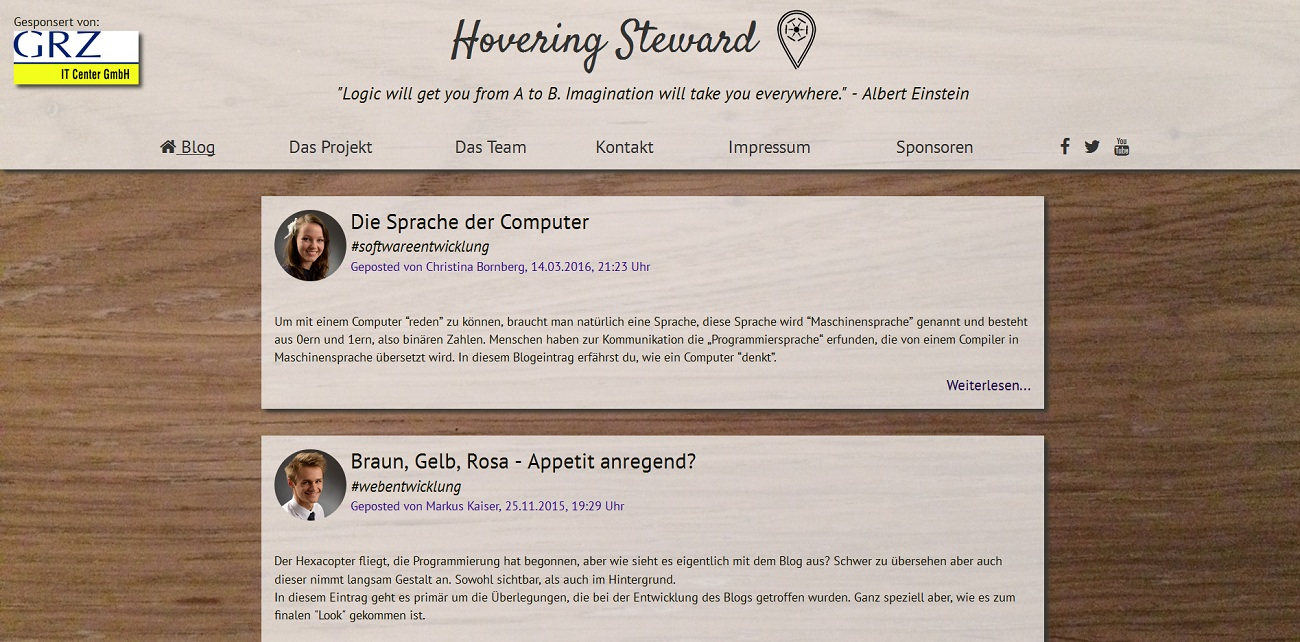
\includegraphics[width = 1\textwidth]{Bilder/blog_dashboard.jpg}
      \par\end{centering}
      \caption{Dashboard des Blogs von Hovering Steward}
      \label{blog}
    \end{figure}

    \subsection*{Frameworks}
    Für die Entwicklung des Blogs erschien der Einsatz eines Frameworks als sehr hilfreich. Das Framework sollte komplexe Methoden wie
    Datenbankzugriffe oder Formularvalidierungen vereinfacht zur Verfügung stellen. Für bessere Übersicht während der Entwicklung war es außerdem
    wichtig, dass das Framework auf dem MVC-Schema aufbaut. Eine Recherche ergab folgende Frameworks als mögliche
    Optionen:

    \begin{itemize}
      \item Laravel
      \item Symfony
      \item CodeIgniter
      \item CakePHP
    \end{itemize}

    Die Wahl fiel auf CodeIgniter, die Begründung dafür ist in Kapitel 1.3.6 angeführt.

  \subsection{Umsetzung}

    \subsection*{Frontend}
    Das Frontend des Blogs setzt sich aus den drei Technologien HTML, JavaScript und CSS zusammen. Aus Gründen von Performance und SEO wurden außerdem
    die JavaScript Bibliothek jQuery und das CSS Framework Bootstrap verwendet. Im Folgenden werden diese Technologien näher beschrieben und die daraus
    ersichtlichen Vorteile, die zu Verwendung in diesem Projekt geführt haben, erläutert.

      \subsubsection*{HTML}
      Die {\textbf{H}yper \textbf{T}ext \textbf{M}arkup \textbf{L}anguage\cite{html}} ist eine gängige Auszeichnungssprache, die verwendet wird um Dokumente mit Text und Medien zu strukturieren.
      Ein HTML-Dokument ist das Grundgerüst einer Website. Ein Webbrowser interpretiert
      HTML und visualisiert dadurch die Website. Die Syntax von HTML besteht aus sogenannten Tags, die, nach einem
      bestimmten Schema aufgebaut, die Struktur einer Website ergeben. Die aktuelle Version ist HTML 5. Diese unterstützt zum einen das responsive
      Entwickeln einer Website, und verbessert zum anderen die SEO (vgl. Abschnitt SEO). Außerdem ist es möglich ohne der Verwendung des Adobe Flash Players Audio und Video einzubinden.

      \subsubsection*{JavaScript}
      {JavaScript\cite{javascript}} ist eine webbasierende Skriptsprache. Sie ist objektorientiert, was bedeutet, dass modular programmiert werden kann, und damit Funktionen oder Eigenschaften
      durch Vererbung einmal geschrieben, und mehrmals wiederverwendet werden können. Die Sprache wird genutzt um eine Website dynamisch, mittels Vorgängen wie Berechnungen oder Animationen auf einer Website durchzuführen.
      Oft sind diese mit Interaktion des Nutzers verbunden. JavaScript greift hierfür auf das Document Object Model des HTML-Dokumtens zu, um Elemente und Knoten in diesem hinzuzufügen, zu löschen, oder
      zu ändern. Ein großer Vorteil von JavaScript ist, dass durch das Einbinden von, auf JavaScript basierenden Bibliotheken, ganz leicht eine Vielzahl von zusätzlichen Funktionen
      verwendet werden können.

      JavaScript ist nachwievor die am weitesten verbreitetste Skriptsprache, die am Client verarbeitet wird. Es wird stark unterstützt, wodurch auch einfach Hilfestellungen im Netz
      gefunden werden können. Es gab daher keinen Grund, eine Alternative zu JavaScript in Betracht zu ziehen.

      Ein gutes Beispiel, und zugleich auch eine, für den Blog verwendete Bibliothek ist {jQuery\cite{jquery}}.
      jQuery ist eine Open-Source Bibliothek, mit dessen Entwicklung versucht wurde, die Nachteile von JavaScript zu beheben. Einer der wesentlichen Vorteile ist
      der vereinfachte Zugriff und die Manipulation von DOM-Elementen.

      Beispiel JavaScript:

      \lstset{language=html}
      	\begin{lstlisting}
          /**
           * Liefert alle <li> Elemente, die sich in einem Element mit der ID "navbar-list" befinden.
          **/
          var list = document.getElementById("navbar-list");
          var items = list.querySelectorAll("li");
      	\end{lstlisting}

      Beispiel: jQuery:

      \lstset{language=html}
      	\begin{lstlisting}
          /**
           * Liefert alle <li> Elemente, die sich in einem Element mit der ID "navbar-list" befinden.
          **/
          var items = $("#navbar-list li");
      	\end{lstlisting}

      Eine derzeit weit verbreitetes JavaScript Framework ist {AngularJS\cite{angular}}. Die Intention dieses Frameworks ist die Automatisierung von oft verwendeten Vorgängen durch
      Datenbindungen und Direktiven. Der Programmierer erspart sich dadurch Codezeilen und Zeit. Zu den sinnvollen Einsatzgebieten von Angular zählen Webseiten mit großteils dynamisch generiertem
      Inhalt oder auch "Single Page Applikations", Webseiten die einmal geladen werden und dann nur zwischen Inhalten wechseln, ohne diese neu zu laden. Das Framework in Kombination mit dem PHP
      Framework CodeIgniter zu verwenden, bedeutete jedoch eine flache Lernkurve. Der Blog war zudem nicht als "Single Page Applikation" geplant, wodurch sich die Verwendung von AngularJS nicht rentiert hätte.

      \subsubsection*{CSS}
      {CSS\cite{css}} steht für \textbf{C}ascading \textbf{S}tyle \textbf{S}heets. Wie das Wort "Style" bereits offenbart, wird sie für das visuelle Aufbereiten einer Website verwendet.
      Allgemein ist CSS eine Gestaltungssprache und wird in Kombination mit HTML-Dokumenten verwendet. In HTML werden dafür den DOM-Elementen Klassen oder IDs
      zugewiesen, über die CSS dann beliegige Eigenschaften zuweisen kann. Dabei orientiert sich CSS nach dem sogenannten Box-Modell. In diesem werden HTML-Elemente
      zwischen Inline-Elementen und Block-Elemente unterschieden. Inline-Elemente passen sich dem Fluss in der Struktur des Dokuments an, Block-Elemente hingegen
      werden für das Layout der Website verwendet. Von einfachen Formatierungen wie der Schriftgröße oder einer Hintergrundfarbe lassen sich mit CSS komlexe Animationen,
      ohne die Verwendung von JavaScript durchführen. Letzteres ist jedoch erst seit der Version CSS3 möglich.

      Das Open-Source Framework {Twitter Bootstrap\cite{bootstrap}} gilt eigentlich als CSS-Framework, da den Elementen die Eigenschaften über CSS Klassen zugewiesen werden, es basiert jedoch
      ebenfalls auf HTML und JavaScript. Neben dem wesentlichen Vorteil der responsiven Gestaltung einer Website, bietet es durch
      zahlreiche, vordefinierte JavaScript Methoden, die ebenfalls durch die Zuweiseung von Klassen an Elemente gebunden werden, die Möglichkeiten, animierte Dropdown-Menüs, Pop-Up-Windows oder Bildergalerien einzubinden.
      Weitere wichtige Eigenschaften von Bootstrap sind die weitreichende Browserkompatibilität und das einheitliche Design.

      Eine Alternative zu Bootstrap stellte {Foundation\cite{foundation}} dar. Es ist ebenso wie Bootstrap ein CSS Framework, mit dem ein responsives Gestalten einer Website umsetzbar ist.
      Da das Framework einen sehr ähnlichen Umfang aufwies fiel die Wahl jedoch auf Bootstrap, da damit bereits öfters gearbeitet wurde und somit weniger Zeitaufwand bedeutete.

    \subsection*{Backend}
    Das Backend setzt sich ausschließlich aus dem Framework CodeIgniter zusammen, welches auf der serverseitigen Scriptsprache PHP basiert. Für die Datenspeicherung
    wurde eine MySQL-Datenbank verwendet.

      \subsubsection*{Code}
        \subsubsection*{PHP}
        {PHP\cite{php}, ausgeschrieben \textbf{P}HP \textbf{H}ypertext \textbf{P}rocessor, ist genau wie JavaScript eine Skriptsprache, mit dem Unterschied, dass der Code nicht auf dem Client, sondern auf dem Server ausgeführt wird,
        und im Anschluss für den Client lesbares HTML generiert. Dies bietet den großen Vorteil, dass für den Client nicht ersichtlich ist, was im Hintergrund an PHP Code ausgeführt
        wird. Um PHP zu programmieren wird allerdings ein Webserver mit einer PHP-Installation benötigt.

        \subsubsection*{Ruby}
        {Ruby\cite{ruby}} ist eine gängie Alternative zu PHP. Neben dem Einsatz in der Webentwicklung wird diese Skriptsprache allerdings auch für allgemeinere Softwareentwicklungsgebiete verwendet.
        Für die Webentwicklung stellt Ruby das Framework {"Ruby on Rails"\cite{rubyonrails}} zur Verfügung.
        Da Ruby jedoch noch keinen so hohen Bekanntheitsgrad wie PHP hat, gibt es weniger ausführlichere Dokumentationen, weswegen PHP als die sinnvollere Variante für das Backend des Blogs erschien.
        Außerdem ist die Überlegung, eine Website in Ruby zu entwickeln damit verbunden, einen geeigneten Webhoster zu finden, welcher über eine Ruby Installation auf dem Server verfügt.

        \subsubsection*{Perl}
        {Perl\cite{perl}} ist ähnlich wie Ruby eine Skriptsprache für vielseitige Nutzung wie Systemadministration, Netzwerkprogrammierung, aber auch Webentwicklung, was sie
        zu einer weiteren Alternative zu PHP macht. Neben dem Vorteil der Plattformunabhängigkeit ist Perl mit den Sprachen HTML und MySQL kompatibel. Beide dieser Sprachen stellen
        einen wichtigen Bestandteil des Blogs dar. Da Perl jedoch im Vergleich zu PHP nicht ausschließlich für die Entwicklung von Webanwendungen vorgesehen ist, sind
        Methodenaufrufe oft viel komplexer, was einen höheren Aufwand bei der Programmierung bedeutet hätte.

      \subsubsection*{Datenbank}

        \subsubsection*{MySQL}
        MySQL ist ein weit verbreitetes relationales Datenbanksystem, das auf SQL basiert. SQL steht für "Structured Query Language" und bezeichnet eine Datenbanksprache.
        Sie wird verwendet um die Struktur einer Datenbank festzulegen, Daten hinzuzufügen, diese zu ändern oder zu löschen. MySQL stellt eine wichtige Schnittstelle zwischen zwei gängigen Sprachen für
        die Enticklung dynamischer Websites zu Verfügung indem sie es ermöglicht, diese Abfragen mit der Scriptsprache PHP durchzuführen. Ein hilfreiches Verwaltungstool ist phpMyAdmin,
        eine in PHP entwickelte Anwendung, die die Verwaltung der MySQL Datenbanken über eine grafische Oberfläche vereinfacht.

        \subsubsection*{MongoDB}
        Anders als MySQL ist {MongoDB\cite{mongodb}} eine NoSQL Datenbank. Der Unterschied liegt darin, dass die Datenbank nicht relational ist. Statt einem konkreten Schema von Tabellen
        wird hier mit sogenannten Dokumenten und Sammlungen gearbeitet. Ein Dokument speichert Daten, nach dem "Key-Value" Prinzip, eine Sammlung enthält mehrere Dokumente.
        Den bedeutendsten Vorteil weist MongoDB in der dynamischen Gestaltung der Datenbank auf. Die Strukturen in Sammlungen können demnach unterschiedlich sein. Die
        Datenübermittlung erfolgt über {BSON\cite{bson}}, ein JSON ähnliches Format, welches im Vergleich zu diesem jedoch auch Datentypen unterstützt.

        Eine Verbindung zu MongoDB über CodeIgniter aufzubauen erwies sich als Nachteil, da zu diesem Zweck eigene Bibliotheken für beispielsweise das Arbeiten mit Sessions
        einzubinden gewesen wären.

    \subsection*{SEO}
    Der Blog war unsere wichtigste Schnittstelle nach Außen, weswegen er im Internet leicht zu finden sein musste. Suchmaschinen wie Google oder Bing nutzen
    sogenannte Robots, kleine Programme, die selbstständig das World Wide Web durchstöbern, um Webseiten zu inspizieren und zu bewerten. Je besser die Bewertung,
    desto weiter oben lässt sich die Website in der Suchmaschine auffinden.
    Die Bewertung hängt von einer Vielzahl von Kriterien ab, von denen folgende bei der Entwicklung des Blogs beachtet wurden:

    \begin{itemize}
      \item \textbf{Aufbau der Seite}

        Die Grundstruktur eines HTML Dokuments besteht aus den drei Teilen:

        \begin{itemize}
          \item Dokumenttyp-Dekleration
          \item head
          \item body
        \end{itemize}

        und sieht wie folgt aus:

        \lstset{language=html}
        	\begin{lstlisting}
            <!DOCTYPE html>
            <html lang="de">
              <head>
                <meta charset="utf-8">
                <meta name="viewport" content="width=device-width, initial-scale=1.0">
                <title>Titel</title>
              </head>
              <body>
              </body>
            </html>
        	\end{lstlisting}

        Ganz oben im Dokument wird der Dokumenttyp deklariert. Dieser gibt die verwendete HTML Version an. Im Falle von HTML 5 würde dieser wie folgt aussehen:

        \lstset{language=html}
        	\begin{lstlisting}
            <!DOCTYPE html>
        	\end{lstlisting}

        Der Dokumenttyp für HTML 4.01 Strict hingegen wurde wie folgt angegeben:

        \lstset{language=html}
        	\begin{lstlisting}
            <!DOCTYPE HTML PUBLIC "-//W3C//DTD HTML 4.01//EN" "http://www.w3.org/TR/html4/strict.dtd">
        	\end{lstlisting}

        Im \textless head \textgreater Bereich werden \textless meta \textgreater Tags angegeben, in denen allgemeine und technische Informationen zur Website, wie Zeichensatz
        und Skalierung bei mobiler Version, oder Keywords und Beschreibung gespeichert werden.
        Die beiden Letzten sind besonders wichtig, da sie dem Robot mitteilen, worum es auf der Seite geht. Er achtet hierbei auch darauf, dass die Beschreibung nicht
        länger als 155 Zeichen lang ist und die Keywords eindeutig gewählt werden.

        Im \textless body \textgreater, also im eigentlichen Inhalt der Website legt der Robot zum einen sehr viel Wert auf Struktur. Beispielsweise muss die Verschachtelung der Tags stimmen,
        oder der \textless h1 \textgreater Tag darf nur einmal pro Seite vorkommen.
        Zum anderen werden Inhalt und Code in Relation gesetzt. Wenn der Aufbau des HTML Dokuments sehr groß ist, in jedem Absatz jedoch nur ein Satz steht, kennt sich der Robot nicht aus.

      \item \textbf{Responsive Design}

        Das Smartphone ist mittlerweile ein ebenso beliebtes Gerät zum Surfen im Internet, wie der Computer. Damit auf dem kleinen Display alles gut lesbar ist, muss die Website speziell
        gestaltet werden. Frameworks wie Bootsrap helfen bei diesem Vorhaben, indem mithilfe von vordefinierten CSS-Klassen die Elemente der Website so gestaltet werden, dass diese mit der
        Bildschirmgröße mitwachsen, sich verschieben oder ausgeblendet werden.

      \item \textbf{Interne und externe Links}

        Bei Links werden sowohl Links, die auf die Website verweisen, als auch Links, die auf andere Seiten zeigen bewertet.
        Zeigen sehr viele externe Links auf eine Seite, interpretiert der Robot diese als geläufig und sie erhält eine höhere Wertung. In unserem Fall war die Kombination mit anderen sozialen
        Medien sehr hilfreich, da durch Veröffentlichungen auf diesen automatisch Links auf unseren Blog generiert werden.

        Links, die von der eigenen Seite auf andere verweisen stellen jedoch einen Nachteil dar, da der Robot dem Link folgen könnte, statt die eigene Seite weiter zu inspizieren. Möchte man dies
        verhindern, kann dem \textless a \textgreater Tag das Attribut rel="nofollow" hinzugefügt werden, um dem Robot zu sagen, dass er diesem Link nicht folgen soll.

      \item \textbf{Sitemap}

      	Die Sitemap ist ein Inhaltsverzeichnis der Website, z.B. in Form einer XML Datei. Die Sitemap hilft dem Robot, wenn er erst einmal auf einer Seite gelandet ist, zugehörige Seiten
        zu finden. Dadurch, dass in der Sitemap die zugehörigen Unterseiten einer Seite mittels URL angegeben werden, hat dies den selben Vorteil wie eine große Anzahl externer Links, die auf diese
        Unterseiten verweisen, nämlich dass Google diese schneller findet. Tools wie xml-sitemaps.com bieten an, eine Sitemap für die angegebene URL zu generieren. Hat der Robot die Seite vollständig
        untersucht, muss die Sitemap im Domain Root-Verzeichnis abgelegt werden. Zuletzt kann die URL zu dieser Sitemap bei Google registriert werden, um Google anzuweisen einen Robot über die Seite
        laufen zu lassen. Nach einigen Tagen sind die Ergebnisse direkt in der Google Suche sichtbar.

      \item \textbf{Browserkompatibilität}

        Nicht jeder Browser stellt jede Seite gleich dar. Die Tags werden unterschiedlich, oder sogar garnicht verstanden. Wird dies nicht beachtet, wirkt sich das auf die Nutzerfreundlichkeit,
        und damit auch auf die Bewertung der Website aus. Um dies zu verhindern gibt es Tools wie zum Beispiel caniuse.com in denen genau verzeichnet ist, welcher Tag, oder welche CSS-Eigenschaft
        von welchem Browser, beziehungsweise welcher Browserversion unterstützt wird.

      \item \textbf{Ladezeit}

        Der Robot bewertet ebenfalls die Ladezeit einer Website. Sie ergibt sich aus der Anzahl an Bildern, Videos oder eingebundenen Bibliotheken oder Schriftarten auf der Website.
        Speziell im Blog, war früh klar, dass viele Bilder geladen werden müssen. Den Upload auf eine niedrige Dateigröße einzuschränken hat zu Beginn nicht ausgereicht.
        Eine Javascript Bibliothek names yoxview hat es allerdings ermöglicht, die Bilder erst dann zu laden, wenn ein Nutzer auf einen Thumbnail klickt. Die Größe der Thumbnails betrugen bloß
        ein paar Kilobyte, wodurch die Ladezeit der Website bedeutend verkürzt werden konnte.

    \end{itemize}

  \subsection{Implementierung}

    \subsection*{FTP Client}
    Für die Verwaltung der Website wurde der Open-Source FTP-Client {FileZilla\cite{filezilla}} verwendet. Ein User kann eine Verbindung zu einem FTP-/SFTP
    Server herstellen, und folglich Verzeichnisse und Dateien auf diesem Server hoch- und herunterladen. {FTP\cite{ftp}} steht für File Transfer Protocol. Es ermöglicht
    den bidirektionalen Austausch von Dateien zwischen Endgeräten. {SFTP\cite{sftp}} bedeutet Secure File Transfer Protocol, nutzt das SSH Protokoll und bietet somit
    einen sichereren Datenaustausch als FTP, da hierbei keine Daten in Klartext, sondern verschlüsselt übertragen werden.

    In Relation zur Notwendigkeit, unsere Dateien zu verschlüsseln, waren die Kosten eines SFTP-Servers jedoch zu hoch, weswegen wir uns für einen einfachen FTP Server entschieden haben.

  \subsection{Herausforderungen und Lösungen}

    \subsection*{Sicherheit}
    Zwei der größten Sicherheitslücken bei Webanwendungen sind zum einen {"Cross-Site-Scripting"\cite{xss}} und zum anderen {"SQL-Injections"\cite{sqlinjections}}.

      \subsubsection*{Cross-Site-Scripting}
      Unter Cross-Site-Scripting, kurz genannt XSS versteht man die Injizierung von schadhaftem Code in eine Webapplikation über eine Schnittstelle, zu der ein User
      einfachen Zugang hat. In den meisten Fällen geschieht dies, wenn ein Nutzer gezielt JavaScript Code über ein Formular auf einer Website in die Anwedung schleust.
      Gelangt dieses Script an einen anderen Enduser, kann es dort beispielsweise ungehindert auf Cookies zugreifen, da der Browser des anderen Endusers nicht weiß,
      dass dem Script nicht zu vertrauen ist.

      Der Beste Weg XSS zu unterbinden ist, die Eingaben, die über ein Formular vom User an den Server gesendet werden über PHP zu validieren und notfalls, Zeichen, die
      XSS andeuten zu ersetzen. PHP stellt dafür die Methode htmlspecialchars() zur Verfügung. Sie konvertiert bestimmte Sonderzeichen in HTML-Code. Beispielsweise wird
      das Zeichen \textless , welches notwendig ist um Javascript mittels \textless script \textgreater-Tag zu schreiben durch "\&lt;" ersetzt.

      \subsubsection*{SQL-Injections}
      Bei einer SQL-Injection hingegen injiziert ein User SQL-Statements in eine Anwedungung um somit Daten aus der Datenbank auszulesen, oder diese zu manipulieren.
      Wird SQL Code dynamisch und mittels User Eingaben generiert, kann der User diese Statements manipulieren. Werden über ein Formular
      geschickte Daten per "\$\_POST['name'];" direkt in ein SQL Statement übernommen, ohne auf korrekte Zeicheneingabe, Länge des Strings oder Ähnliches validiert wird,
      können Fehler entstehen, die Schaden an der Datenbank anrichten.

      Eine Möglichkeit eine SQL Injection zu verhindern ist, ähnlich wie bei XSS bestimmte Zeichen zu erkennen und stattdessen als Strings weiterzuverwenden.
      Mit einem einfachen Hochkomma ist es möglich einen Wert zu unterbrechen, und an dieser Stelle SQL-Code einzufügen, die die Abfrage beeinflussen.
      Mit der PHP Methode mysql\_real\_escape\_string() wird vor jedes Zeichen wie zum Beispiel ein ' ein \textbackslash geschrieben, womit dieses zu einem ganz normalen
      String Ausdruck wird, und damit ungefährlich ist.

    \subsection*{Responsive Design}
    Für die responsive Gestaltung des Blogs wurde zwar das Framework Bootstrap herangezogen, da der Aufbau der Website jedoch aus eigener Hand
    entstanden ist, und kein Template verwendet wurde, musste für vollständige Kompatibilität auf mobilen Geräten manuell mit CSS gearbeitet werden.
    Mittels Media-Queries lassen sich CSS-Eigenschaften so definieren, dass sie ab gewissen Bildschirmgrößen aktiv werden. Für die Bildschirmbreiten 1200, 992, 767 und 480
    Pixel wurden verschiedene CSS-Eigenschaften definiert. Diese vier Größen sind von Bootstrap hergeleitet und teilen Geräte in die vier Typen Phones, Tablets,
    Desktop und Large Desktop.

  \subsection{Persönliche Erfahrungen}
    \subsection*{Eigenes CMS}
    Durch die Verwendung der Content Management Systeme TYPO3 und Wordpress im Unterricht, war ich bereits mit diesem Themengebiet vertraut. Was mich speziell interessiert hat war,
    was hinter einem CMS steckt. Ich wollte die Abläufe und verschiedenen Schritte kennen und habe mich aus diesem Grund entschieden den Blog als eigenes Content Management System
    zu entwickeln. Aus zeitlichen Gründen sollte es allerdings nur die Funktionen einer Nutzerverwaltung und einer Beitragveröffentlichung unterstützen.

    \subsection*{Wahl des Frameworks}
    Die Recherche ergab, dass mehrere, unterschiedlich umfangreiche PHP Frameworks für den Blog geeignet wären. Da nicht genug Zeit war jedes testweise zu installieren und
    sich mit den Grundlagen auseinanderzusetzen, habe ich mich an Rezensionen von Nutzern dieser Frameworks orientiert. CodeIgniter stellte sich als optimales Framework für
    die Entwicklung einer Webanwendung dieser Größe heraus. Es bietet zahlreiche Bibliotheken, die über sehr simple Einbindung die Funktionalitäten erweitern. Syntaktisch ist
    das Framework meiner Meinung nach außerdem einfacher zu lernen als PHP ansich. Eine Installation war auch nicht notwendig. Die Ordnerstruktur musste nach dem Download nur
    exportiert, und in einem Projektordner von XAMPP eingefügt werden. Der Vorbereitungsprozess war dadurch, und zusätzlich dank einer besonders guten Dokumentation minimal.
